\documentclass[a4paper]{report}
\usepackage[utf8]{inputenc}
\usepackage[T1]{fontenc}
\usepackage{RJournal}
\usepackage{amsmath,amssymb,array}
\usepackage{booktabs}


% tightlist command for lists without linebreak
\providecommand{\tightlist}{%
  \setlength{\itemsep}{0pt}\setlength{\parskip}{0pt}}


% Always define CSL refs as bib entries are contained in separate doc
% Pandoc citation processing
\newlength{\cslhangindent}
\setlength{\cslhangindent}{1.5em}
\newlength{\csllabelwidth}
\setlength{\csllabelwidth}{3em}
\newlength{\cslentryspacingunit} % times entry-spacing
\setlength{\cslentryspacingunit}{\parskip}
% for Pandoc 2.8 to 2.10.1
\newenvironment{cslreferences}%
  {}%
  {\par}
% For Pandoc 2.11+
\newenvironment{CSLReferences}[2] % #1 hanging-ident, #2 entry spacing
 {% don't indent paragraphs
  \setlength{\parindent}{0pt}
  % turn on hanging indent if param 1 is 1
  \ifodd #1
  \let\oldpar\par
  \def\par{\hangindent=\cslhangindent\oldpar}
  \fi
  % set entry spacing
  \setlength{\parskip}{#2\cslentryspacingunit}
 }%
 {}
\usepackage{calc}
\newcommand{\CSLBlock}[1]{#1\hfill\break}
\newcommand{\CSLLeftMargin}[1]{\parbox[t]{\csllabelwidth}{#1}}
\newcommand{\CSLRightInline}[1]{\parbox[t]{\linewidth - \csllabelwidth}{#1}\break}
\newcommand{\CSLIndent}[1]{\hspace{\cslhangindent}#1}



\begin{document}


%% do not edit, for illustration only
\sectionhead{Contributed research article}
\volume{XX}
\volnumber{YY}
\year{20ZZ}
\month{AAAA}

\begin{article}
  % !TeX root = RJwrapper.tex
\title{Frame to frame interpolation for high-dimensional data
visualisation using the woylier package}
\author{by Zoljargal Batsaikhan, Dianne Cook, and Ursula Laa}

\maketitle

\abstract{%
The woylier package implements tour interpolation paths between frames
using Givens rotations. This provides an alternative to the geodesic
interpolation between planes currently available in the tourr package.
Tours are used to visualise high-dimensional data and models, to detect
clustering, anomalies and non-linear relationships. Frame-to-frame
interpolation can be useful for projection pursuit guided tours when the
index is not rotationally invariant. It also provides a way to
specifically reach a given target frame. We demonstrate the method for
exploring non-linear relationships between currency cross-rates.
}

\hypertarget{introduction}{%
\section{Introduction}\label{introduction}}

When data has up to three variables, visualization is relatively
intuitive, while with more than three variables, we face the challenge
of visualizing high dimensions on 2D displays. This issue was tackled by
the \emph{grand tour} \citep{asimov_1985} which can be used to view data
in more than three dimensions using linear projections. It is based on
the idea of rotations of a lower-dimensional projection in
high-dimensional space. The grand tour allows users to see dynamic
low-dimensional (typically 2D) projections of higher dimensional space.
Originally, Asimov's grand tour presents the viewer with an automatic
movie of projections with no user control. Since then new work has added
interactivity to the tour, giving more control to users
\citep{buja_cook_asimov_hurley_2005}. New variations include the manual
\citep{cook_manual_1997} or radial tour \citep{mmtour}, little tour,
guided tour \citep{grandtour1995}, local tour, and planned tour. These
are different ways of selecting the sequence of projection bases for the
tour, for an overview see \citet{tourrev}.

The guided tour combines projection pursuit with the grand tour and it
is implemented in the \CRANpkg{tourr} package \citep{tourr}. Projection
pursuit is a procedure used to locate the projection of high-to-low
dimensional space that should expose the most interesting feature of
data, originally proposed in \citet{kruskal_1969}. It involves defining
a criterion of interest, a numerical objective function that indicates
the interestingness of each projection, and an optimization for
selecting planes with increasing values of the function. In the
literature, a number of such criteria have been developed based on
clustering, spread, and outliers.

A tour path is a sequence of projections and we use an interpolation to
produce small steps simulating a smooth movement. The current
implementation of tour in the \CRANpkg{tourr} package uses geodesic
interpolation between planes. The geodesic interpolation path is the
shortest path between planes with no within-plane spin (see
\citet{Buja2004TheoryOD} for more details). As a result, the rendered
target plane could be a within-plane rotation of the target plane
originally specified. This is not a problem when the structure we are
looking for can be identified from any rotation. However, even simple
associations in 2D, such as the calculated correlation between
variables, can be very different when the basis is rotated.

Most projection pursuit indexes, particularly those provided by in
\CRANpkg{tourr} are rotationally invariant. However, there are some
where the orientation of frames does matter. One example is the splines
index proposed by \citet{Grimm2016}. The splines index computes a spline
model for the two variables in a projection, in order to measure
non-linear association. It compares the variance of the response
variable to the variance of residuals, and the functional dependence is
stronger when the index value is larger. It can be useful to detect
non-linear relationships in high-dimensional data. However, its value
will change substantially if the projection is rotated within the plane
\citep{pp}. The procedure in \citet{Grimm2016} was less affected by the
orientation because it considered only pairs of variables, and it
selects the maximum value found when exchanging which variable is
considered as predictor and response variable.

Figure \ref{fig:splines2d-static} illustrates the rotational invariance
problem for a modified splines index, where we always consider the
horizontal direction as the predictor variable, and the vertical
direction as the response. Thus, our modified index computes the splines
on one orientation, exaggerating the rotational variability. The example
data was simulated to follow a sine curve and the modified splines index
is calculated on different within-plane rotations of the data. Although
they have the same structure, the index values vary greatly.

The lack of rotation invariance of the splines index raises
complications in the optimisation process in the projection-pursuit
guided tour as available in \CRANpkg{tourr}. Fixing this is the
motivation of this work. The goal with the frame-to-frame interpolation
is that optimisation would find the best within-plane rotation, and thus
appropriately optimize the index.

\begin{Schunk}
\begin{figure}
\includegraphics[width=1\linewidth]{woylier-article_files/figure-latex/splines2d-static-1} \caption[The impact of rotation on a spline index that is NOT rotation invariant]{The impact of rotation on a spline index that is NOT rotation invariant. The index value for different within-plane rotations take very different values: (a) original projection has maximum index value of 1.00, (b) axes rotated 45$^o$ drops index value to 0.83, (c) axes rotated 60$^o$ drops index to a very low 0.26. Geodesic interpolation between planes will have difficulty finding the maximum of an index like this because it is focused only on the projection plane, not the frame defining the plane.}\label{fig:splines2d-static}
\end{figure}
\end{Schunk}

A few alternatives to geodesic interpolation were proposed by
\citet{buja_cook_asimov_hurley_2005} including the decomposition of
orthogonal matrices, Givens decomposition, and Householder
decomposition. The purpose of the \textbf{woylier} package is to
implement the Givens paths method in R. This algorithm adapts the
Given's matrix decomposition technique which allows the interpolation to
be between frames rather than planes.

This article is structured as follows. The next section provides the
theoretical framework of the Givens interpolation method followed by a
section about the implementation in R. The method is applied to search
for nonlinear associations between currency cross-rates.

\hypertarget{background}{%
\section{Background}\label{background}}

The tour method of visualization shows a movie that is an animated
high-to-low dimensional data rotation. It is a one-parameter (time)
family of static projections. Algorithms for such dynamic projections
are based on the idea of smoothly interpolating a discrete sequence of
projections \citep{buja_cook_asimov_hurley_2005}.

The topic of this article is the construction of the paths of
projections. The interpolation of these paths can be compared to
connecting line segments that interpolate points in Euclidean space.
Interpolation acts as a bridge between a continuous animation and the
discrete choice of sequences of projections.

\textbf{Interpolating paths of planes versus paths of frames}

The \CRANpkg{tourr} package implements geodesic interpolation between
planes, and the final interpolation step will reach the rotation of the
target frame that is avoiding any within-plane spin along the path. When
the the orientation of projections matters interpolation between frames
is required. The orientation of the frames could be important when a
non-linear projection pursuit index function is used in the guided tour.
This is illustrated by the different index values shown in the sketch in
Figure \ref{fig:dogs}, as well as the splines index for the sine curve
in Figure \ref{fig:splines2d-static}.

XXX I like the dog sketch but currently seems not really needed - what
would be nice would be showing a bit more here: starting plane is the
dog looking in a different direction and also at an angle, target is the
one aligned as currently seen in the front, geodesic path gets us to the
target view at the angle as seen in the starting plane, givens path
gives the exact target. Not sure how difficult it would be to make this
though\ldots{}

\begin{Schunk}
\begin{figure}

{\centering 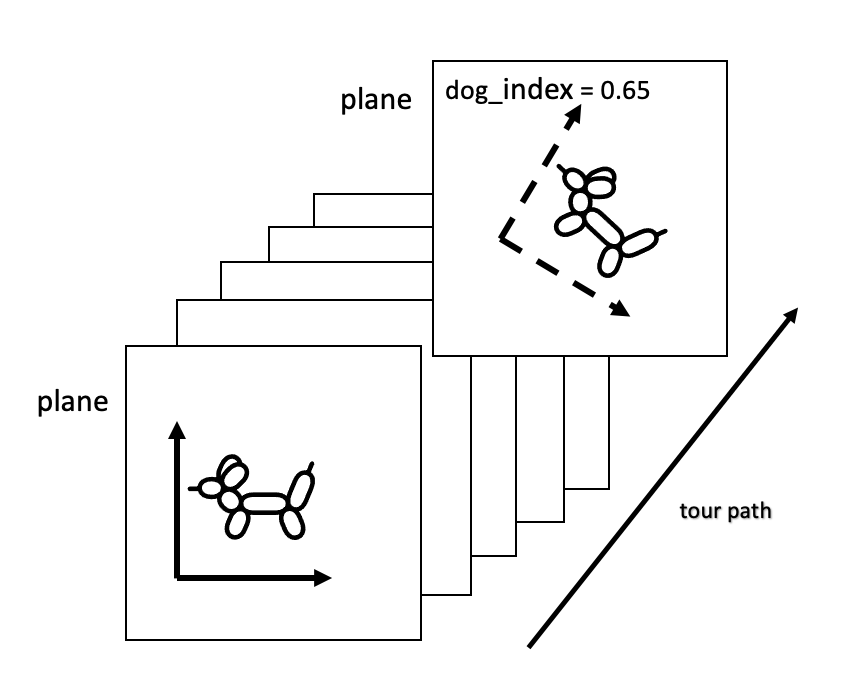
\includegraphics[width=0.45\linewidth]{plane} 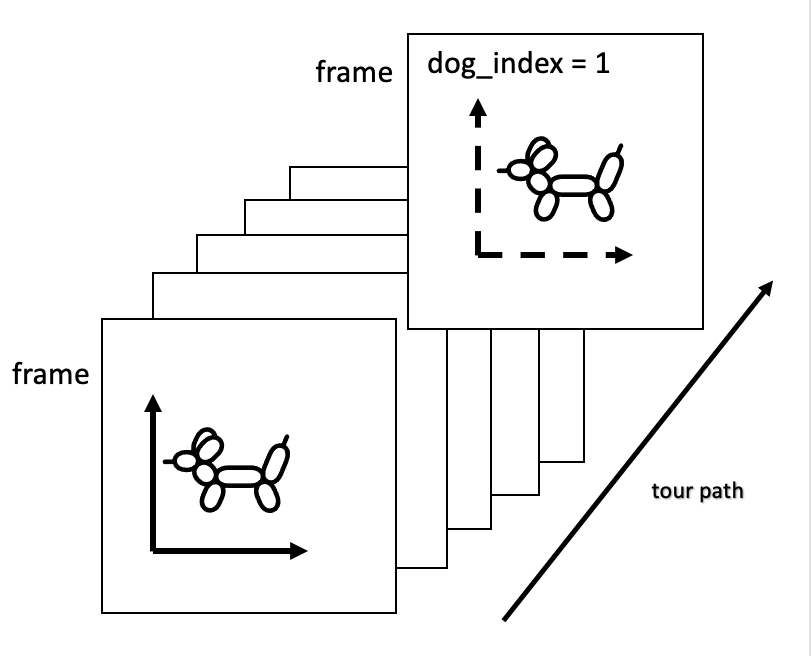
\includegraphics[width=0.45\linewidth]{frame} 

}

\caption[Plane to plane interpolation (left) and Frame to frame interpolation (right)]{Plane to plane interpolation (left) and Frame to frame interpolation (right). We used dog index for illustration purposes. For some non-linear index orientation of data could affect the index.}\label{fig:dogs}
\end{figure}
\end{Schunk}

To describe the interpolation algorithms we will use the following
notation.

\begin{itemize}
\item
  Let \(p\) be the dimension of original data and \(d\) be the dimension
  onto which the data is being projected.
\item
  A frame \(F\) is defined as a \(p\times d\) matrix with pairwise
  orthogonal columns of unit length that satisfies \[F^TF = I_d,\] where
  \(I_d\) is the identity matrix in d dimensions.
\item
  Paths of frames are given by continuous one-parameter families
  \(F(t)\) where \(t\in [a, z]\) represents time. We denote the starting
  frame (at time \(a\)) by \(F_a = F(a)\) and target frame (at time
  \(z\)) by \(F_z = F(z)\). Usually, \(F_z\) is the target frame that
  has been chosen according to the selected tour method. While a grand
  tour chooses target frames randomly, the guided tour chooses the
  target frame by optimizing the projection pursuit index. Interpolation
  methods are used to find the path that moves from \(F_a\) to \(F_z\).
\end{itemize}

\textbf{Preprojection algorithm}

In order to make the interpolation algorithm simple, we carry out a
preprojection step to find the subspace that the interpolation path,
\(F(t)\), is traversing. In other words, the preprojection step is
defining the joint subspace of \(F_a\) and \(F_z\) and makes sure the
interpolation path is limited to that space.

The procedure starts with forming an orthonormal basis by applying
Gram-Schmidt to \(F_z\) with regards to \(F_a\), i.e.~we find the
\(p\times d\) matrix that contains the component of \(F_z\) that is
orthogonal to \(F_a\). We denote this orthonormal basis by \(F_\star\).
Then we build the preprojection basis \(B\) by combining \(F_a\) and
\(F_\star\) as follows:

\[B = (F_a, F_{\star})\]

The dimension of the resulting orthonormal basis, \(B\), is
\(p\times 2d\).

Then, we can express the original frames in terms of this basis:

\[F_a = B W_a, F_z = B W_z\]

The interpolation problem is then reduced to the construction of paths
of frames \(W(t)\) that interpolate between the preprojected frames
\(W_a\) and \(W_z\). By construction \(W_a\) is a \(2d\times d\) matrix
of 1s and 0s. This is an important characteristic for our interpolation
algorithm of choice, the Givens interpolation.

\textbf{Givens interpolation path algorithm}

A rotation matrix is a transformation matrix used to perform a rotation
in Euclidean space. The matrix that rotates a 2D plane by an angle
\(\theta\) looks like this:

\[ \begin{bmatrix}\cos \theta &-\sin \theta \\\sin \theta &\cos \theta \end{bmatrix} \]

If the rotation is in the plane of two selected variables, it is called
a Givens rotation. Let's denote those 2 variables as \(i\) and \(j\).
The Givens rotation is used for introducing zeros, for example when
computing the QR decomposition of a matrix in linear algebra problems.

The interpolation method in the \textbf{woylier} package is based on the
fact that in any vector of a matrix, one can zero out the \(i\)-th
coordinate with a Givens rotation in the \((i, j)\)-plane for any
\(j\neq i\) \citep{matrix_computation}. This rotation affects only
coordinates \(i\) and \(j\) and leaves all other coordinates unchanged.
Sequences of Givens rotations can map any orthonormal d-frame \(F\) in
p-space to the standard d-frame
\[E_d=((1, 0, 0, ...)^T, (0, 1, 0, ...)^T, ...).\]

The resulting interpolation path construction algorithm from starting
frame \(F_a\) to target frame \(F_z\) is illustrated below. The example
is for \(p=6\) and \(d=2\).

\begin{enumerate}
\def\labelenumi{\arabic{enumi}.}
\tightlist
\item
  Construct preprojection basis \(B\) by orthonormalizing \(F_z\) with
  regards tp \(F_a\) with Gram-Schmidt.
\end{enumerate}

In our example, \(F_a\) and \(F_z\) are \(p\times d\) or \(6\times2\)
matrices that are orthonormal. The preprojection basis \(B\) is
\(p\times 2d\) matrix that is \(6\times 4\).

\begin{enumerate}
\def\labelenumi{\arabic{enumi}.}
\setcounter{enumi}{1}
\tightlist
\item
  Get the preprojected frames using the preprojection basis \(B\).
  \[W_a = B^TF_a = E_d\] and \[W_z = B^TF_z\]
\end{enumerate}

In our example, \(W_a\) looks like:

\[ \begin{bmatrix}1 & 0 \\0  &1 \\ 0&0 \\0&0\end{bmatrix} \]

\(W_z\) is an orthonormal \(2d\times d\) matrix that looks like:

\[ \begin{bmatrix} a_{11} & a_{12} \\a_{21}  &a_{22} \\ a_{31}&a_{32} \\a_{41}&a_{42}\end{bmatrix} \]

\begin{enumerate}
\def\labelenumi{\arabic{enumi}.}
\setcounter{enumi}{2}
\tightlist
\item
  Then, we can construct a sequence of Givens rotations that maps
  \(W_z\) to \(W_a\) with such angles that makes one element zero at a
  time:
\end{enumerate}

\[ W_a = R_m(\theta_m) ... R_2(\theta_2)R_1(\theta_1)W_z\]

At each rotation, the angle \(\theta_i\) that zero out the next
coordinate of a plane is calculated. Here \(m = \sum_{k=1}^d (2d - k)\),
so when \(d=2\) we need \(m=5\) rotations with 5 different angles, each
making one element 0. For example, the first rotation angle \(\theta_1\)
is an angle in radiant between \((1, 0)\) and \((a_{11}, a_{21})\). This
rotation matrix would make element \(a_{21}\) zero:

\[R_1(\theta_1) = G(1, 2, \theta_1) = \begin{bmatrix} cos\theta_1 & -sin\theta_1 & 0 & 0 \\sin\theta_1  &cos\theta_1 & 0 &0 \\ 0&0&1&0 \\0&0&0&1\end{bmatrix}\]
Here \(G(i,j,\theta_k)\) denotes a Givens rotation in components \(i\)
and \(j\) by angle \(\theta_k\). In the same way we zero out the
elements \(a_{31}\) and \(a_{41}\). Because of the orthonormality this
means that now \(a_{11} = 1\) and that \(a_{12} = 0\). We thus need only
two more rotations to zero out \(a_{32}\) and \(a_{42}\).

XXX something about how we calculate theta?

\begin{enumerate}
\def\labelenumi{\arabic{enumi}.}
\setcounter{enumi}{3}
\tightlist
\item
  The inverse mapping is obtained by reversing the sequence of rotations
  with the negative of the angles, we starts from the starting basis and
  end at the target basis.
\end{enumerate}

\[R(\theta) = R_1(-\theta_1) ... R_m(-\theta_m), \    W_z = R(\theta)W_a\]

Performing these rotations would go from the starting frame to the
target frame in one step. But we want to do it sequentially in a number
of steps so interpolation between frames looks dynamic.

\begin{enumerate}
\def\labelenumi{\arabic{enumi}.}
\setcounter{enumi}{4}
\item
  Next we include the time parameter, \(t\), so that the interpolation
  process can be rendered in the movie-like sequence. We break each
  \(\theta_k\) into the number of steps, \(n_{step}\), that we want to
  take from the starting frame to the target frame, which means it moves
  by equal angle in each step. Here \(n_{step}\) should vary based on
  the angular distance between \(F_a\) and \(F_z\), such that when
  watching a sequence of interpolations we have a fixed angular speed.
\item
  Finally, we reconstruct our original frames using \(B\). This
  reconstruction is done at each step of interpolation so that we have
  the interpolated path of frames as the result.
\end{enumerate}

\[F_t = B  W_t\]

At each time \(t\) we can project the data using the frame \(F_t\).

\hypertarget{implementation}{%
\section{Implementation}\label{implementation}}

We implemented each steps in the Givens interpolation path algorithm in
separate functions and combined them in the
\texttt{givens\_full\_path()} function for deriving the full set of
\(F_t\). The same functions are used to integrate the Givens
interpolation with the \texttt{animate()} functions of the
\CRANpkg{tourr} package. Here is the input and output of each functions
and it's descriptions, functions to use with \texttt{animate()} are
described separately below.

\begin{tabular}[t]{>{\raggedright\arraybackslash}p{5cm}|>{\raggedright\arraybackslash}p{3cm}|>{\raggedright\arraybackslash}p{2cm}|>{\raggedright\arraybackslash}p{2cm}}
\hline
\textbf{name} & \textbf{description} & \textbf{input} & \textbf{output}\\
\hline
\ttfamily{givens\_full\_path(Fa, Fz, nsteps)} & Construct full interpolated frames. & Starting and target frame (Fa, Fz) and number of steps & An array with nsteps matrix. Each matrix is interpolated frame in between starting and target frames.\\
\hline
\ttfamily{preprojection(Fa, Fz)} & Build a d-dimensional pre-projection space by orthonormalizing Fz with regard to Fa. & Starting and target frame (Fa, Fz) & B pre-projection p x 2D matrix\\
\hline
\ttfamily{construct\_preframe(Fa, B)} & Construct preprojected frames. & A frame and the pre-projection p x 2D matrix & Pre-projected frame in pre-projection space\\
\hline
\ttfamily{row\_rot(a, i, k, theta)} & Performs Givens rotation . & A frame and the pre-projection p x 2D matrix & theta angle rotated matrix a\\
\hline
\ttfamily{calculate\_angles(Wa, Wz)} & Calculate angles of required rotations to map Wz to Wa. & Preprojected frames (Wa, Wz) & Names list of angles\\
\hline
\ttfamily{construct\_moving\_frame(Wt, B)} & Reconstruct interpolated frames using pre-projection. & Pre-projection matrix B, Each frame of givens path & A frame of on a step of interpolation\\
\hline
\end{tabular}

When using \CRANpkg{tourr} we typically want to run a tour live, such
that target selection and interpolation are interleaved, and the display
will show the data for each frame \(F_t\) in the interpolation path. The
implementation in \CRANpkg{tourr} was described in \citet{tourr}, and
with \CRANpkg{woylier} we provide functions to use the Givens
interpolation with the grand tour, guided tour and planned tour. To do
this we rely primarily on the function \texttt{givens\_info()} which
calls the functions listed in the Table above and collects all necessary
information for interpolating between a given starting and target frame.
The function \texttt{givens\_path()} then defines the interpolation and
can be used instead of \texttt{tourr::geodesic\_path()}. Wrapper
functions for the different tour types are available to use this
interpolation, since in the \texttt{tourr::grand\_tour()} and other path
functions this is fixed to use the geodesic interpolation. Calling a
grand tour with Givens interpolation for direct animation will then use:

\begin{Schunk}
\begin{Sinput}
tourr::animate_xy(<data>, tour_path = woylier::grand_tour_givens())
\end{Sinput}
\end{Schunk}

\hypertarget{comparison-of-geodesic-interpolation-and-givens-interpolation}{%
\section{Comparison of geodesic interpolation and Givens
interpolation}\label{comparison-of-geodesic-interpolation-and-givens-interpolation}}

The \texttt{givens\_full\_path()} function returns the intermediate
interpolation step projections for a given number of steps. The code
chunk below demonstrates the interpolation between 2 random bases in 5
steps.

XXX maybe drop the printout of base1 and base2 since output is not shown
anyways?

\begin{Schunk}
\begin{Sinput}
set.seed(2022)
p <- 6
base1 <- tourr::basis_random(p, d=2)
base2 <- tourr::basis_random(p, d=2)

base1
base2
\end{Sinput}
\end{Schunk}

\begin{Schunk}
\begin{Sinput}
givens_full_path(base1, base2, nsteps = 5)
\end{Sinput}
\end{Schunk}

To compare the path generated with the Givens interpolation to that
found with geodesic interpolations we look at the rotation of the sine
data shown in Figure \ref{fig:splines2d-static}. We consider a subset in
\(p=4\) dimensions where the first two dimensions contain noise and the
last two contain the sine curve. Starting from a random projection we
want to interpolate towards the original sine curve. The path comparison
is shown in Figure \ref{fig:compare-paths}.

\begin{Schunk}
\begin{figure}

{\centering 
\includegraphics[width=0.8\linewidth]{compare-paths} 

}

\caption[Comparison of Givens path and geodesic path between 2D projections]{Comparison of Givens path and geodesic path between 2D projections. The Givens path preserves the frame ending at the provided basis (frame), while geodesic is agnostic to the particular basis. In general the geodesic is preferred because it removes within-plane spin, but occasionally it is helpful to very specifically arrive at the prescribed basis.}\label{fig:compare-paths}
\end{figure}
\end{Schunk}

\textbf{Plotting the interpolated paths}

For further comparison and to check that the interpolation is moving in
equally sized steps we directly plot the interpolated paths. The space
of 1D projections defines a unit sphere, while 2D projections define a
torus. To illustrate the space, points on the surface of the sphere and
the torus shape are randomly generated by functions from the
\CRANpkg{geozoo} package \citep{geozoo}. The interpolated paths are then
compared within that space.

A 1D projection of data in \(p\) dimensions corresponds to a linear
combination where the weights are normalized. Therefore, we can plot the
point on the surface of a hypersphere. In this case the Givens
interpolation will reach the exact point, while geodesic interpolation
might flip the direction and reach a point on the opposite side of the
hypersphere. Figure \ref{fig:1d-path-static} (left) shows the comparison
of the interpolation steps using the same target plane, for an example
with \(p=3\). Because the flipped target is close to the starting plane,
the geodesic path is a lot shorter.

\begin{Schunk}
\begin{figure}

{\centering 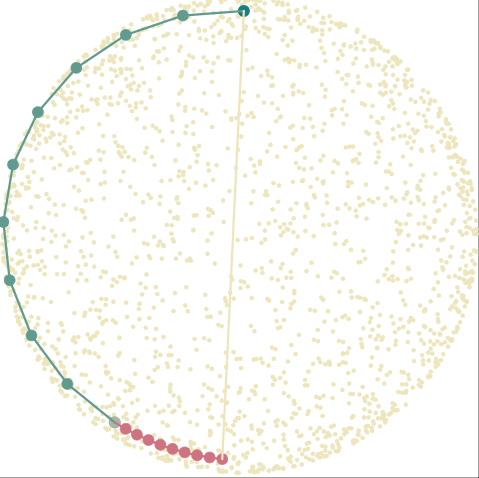
\includegraphics[width=0.45\linewidth]{sphere_static} 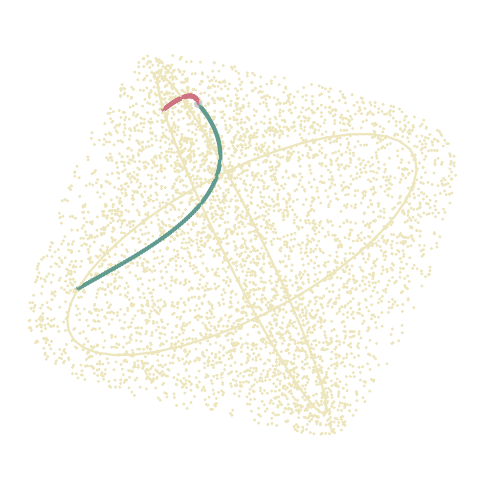
\includegraphics[width=0.45\linewidth]{torus_static} 

}

\caption[Interpolation steps of 1D (left) and 2D (right) projections of 3D data made with a Givens path (forest green) and a geodesic path (deep red)]{Interpolation steps of 1D (left) and 2D (right) projections of 3D data made with a Givens path (forest green) and a geodesic path (deep red). The cream points represent the space of all projections, which is a sphere for 1D projections and a torus for 2D projections. In the 1D example, geodesic arrives at the opposite side of the sphere to Givens, indicating that it has flipped the direction of the vector in order to make the shortest path to the same plane. A similar thing happens for the 2D example, geosesic flips the sign of one basis vector, but it defines the same plane, as indicated by the cream circles.}\label{fig:1d-path-static}
\end{figure}
\end{Schunk}

In case of 2D projections, we can plot the interpolated path between 2
frames on a torus. A torus can be seen as crossing of 2 circles that are
orthonormal, as is the case with our projection onto 2D. Figure
\ref{fig:1d-path-static} (right) compares the interpolation paths for
\(p=3\).

For a 2D projection the same target plane is found when rotating the
basis within the plane, or when reflecting across one of the two
directions (the reflected basis can then also be rotated). This means
the space of target bases is constrained to two circles on the torus,
and these are disconnected because the reflection corresponds to a jump.
In the high-dimensional space we can imagine the reflection as flipping
over the target plane, resulting in a reflection of the normal vector on
the plan. While the Givens interpolation will reach the exact basis, a
geodesic interpolation towards the same target plane can land anywhere
along those two circles, depending on the starting basis in the
interpolation.

\hypertarget{data-application}{%
\section{Data application}\label{data-application}}

This section describes the application of Givens interpolation path with
guided tour to explore non-linear association in multivariate data. We
use cross-rates for currencies relative to the US dollar. A cross-rate
is an exchange rate between two currencies computed by reference to a
third currency, usually the US dollar.

The data was extracted from
\href{https://openexchangerates.org}{openexchangerates} and contains
cross-rate for ARS, AUD, EUR, JPY, KRW, MYR between 2019-11-1 to
2020-03-31. Figure \ref{fig:currency} shows how the currencies changed
relative to USD over the time period. We see some collective behavior in
March of 2020 with EUR and JPY increasing in a similar manner, and
smaller currencies decreasing in value. This could be understood as a
consequence of flight-to-quality at this uncertain times.

\begin{Schunk}
\begin{figure}
\includegraphics[width=1\linewidth]{woylier-article_files/figure-latex/currency-1} \caption[All the currencies are standardised and the sign is flipped]{All the currencies are standardised and the sign is flipped. The high value means the currency strengthened against the USD, and low means that it weakened.}\label{fig:currency}
\end{figure}
\end{Schunk}

We are interested in capturing this relations over time, and from the
time series visualization we expect that we can capture the main
dynamics in a two-dimensional projection from the six-dimensional space
of currencies. Thus we start from \(p=6\) (the different currencies) and
\(n=152\) the number of days in our sample. We expect that a projection
onto \(d=2\) dimensions should capture the relation between the two
groups of currencies mentioned above, and this should be identified
within the noise of the random fluctuations.

We may expect that we can capture the dependence between the two groups
using principal components analysis. Figure \ref{fig:pca-result-static}
shows a scatter plot matrix of the PCs of our dataset. Indeed we find
strong non-linear association between the first two PCs. Investigation
of the rotation shows that the first principal component is primarily a
balanced combination between ARS, AUD, KRW and MYR (and a smaller
contribution of EUR), and the second contribution is dominated by EUR
and JPY contrasted with smaller contributions from ARS and MYR. Our next
step is thus to use projection pursuit to identify the best projection
matrix that captures the non-linear functional dependence.

\begin{Schunk}
\begin{figure}

{\centering \includegraphics[width=0.8\linewidth]{woylier-article_files/figure-latex/pca-result-static-1} 

}

\caption[There is a strong non-linear dependence between PC1 and PC2]{There is a strong non-linear dependence between PC1 and PC2. Observations in March 2020 are highlighted in dark blue, all other months are shown in grey.}\label{fig:pca-result-static}
\end{figure}
\end{Schunk}

\textbf{Guided tour optimisation}

We now use the splines index to identify a projection with functional
dependence between the first and second direction of the projection.
Note here that because of strong linear correlations between the
currencies, we start from the first four principal components,
explaining over 97\% of the variance in the data. To avoid starting from
the view already identified in the first two principal components we
start from a projections onto the third and forth principal components.
The PCA display in \texttt{tourr} is used to show each projection axes
display in terms of the original variables, while only touring within
the smaller space spanned by the first four principal components.

The results are shown in Figure \ref{fig:rates-tour-static} and we see
on the right that the guided tour with Givens interpolation has
identified a non-linear functional dependence between the x and y axis
in the final projection. The result on the left is using geodesic
optimization, and the result in the middle is using a random search with
geodesic interpolation. Since these methods do not allow for
within-plane rotation they were not able to identify the same view even
though they are using the same starting plane and index function.

\begin{Schunk}
\begin{figure}

{\centering 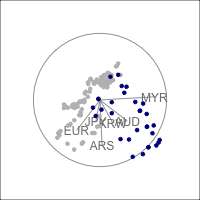
\includegraphics[width=0.3\linewidth]{rates_tour_geodesic_final} 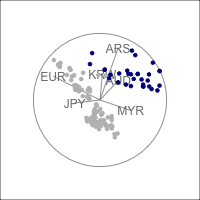
\includegraphics[width=0.3\linewidth]{rates_tour_better_final} 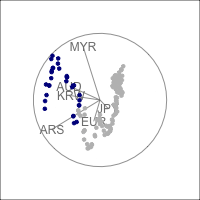
\includegraphics[width=0.3\linewidth]{rates_tour_givens_final} 

}

\caption[Final view after optimisation in the guided tour using geodesic optimisation (left), simulated annealing with geodesic interpolation (middle) and simulated annealing with givens interpolation (right)]{Final view after optimisation in the guided tour using geodesic optimisation (left), simulated annealing with geodesic interpolation (middle) and simulated annealing with givens interpolation (right).}\label{fig:rates-tour-static}
\end{figure}
\end{Schunk}

To understand the result in more detail we use tools from
\CRANpkg{ferrn} \citep{ferrn} to show how the index value is changing
over the optimization in Figure \ref{fig:rates-ferrn}. Points indicate
selected target planes, and are connected by lines showing the index
value along the interpolated path between them.

The top row is showing the path found via geodesic optimization. This
search strategy only moves along geodesic paths, and cannot select
target frames with rotation within the plane. We can see that as a
consequence the optimization converges to a local optimum and the search
does not identify the pattern of interest.

In the middle we are showing the path found when using a random search
in combination with geodesic interpolation. In this case the search can
suggest any target frame (allowing for within-plane rotation), but the
interpolation step will reset the orientation. This is why we see drops
in the index value even from one target plane to the next, and the
optimization also does not identify the pattern of interest.

Finally in the bottom row we see the result of the random search with
Givens interpolation. While the index value can drop along an
interpolation path, the value is strictly increasing for the target
planes, as is required for the optimization. Note also that the search
converged much faster (fewer target planes were selected). The length of
the interpolated paths is similar, because for fixed angular step size
the Givens interpolation will take more steps to interpolate between
frames.

\begin{Schunk}
\begin{figure}
\includegraphics{woylier-article_files/figure-latex/rates-ferrn-1} \caption[Splines index value along the interpolated optimisation path in the guided tour using geodesic optimisation (top), simulated annealing with geodesic interpolation (middle) and simulated annealing with givens interpolation (bottom)]{Splines index value along the interpolated optimisation path in the guided tour using geodesic optimisation (top), simulated annealing with geodesic interpolation (middle) and simulated annealing with givens interpolation (bottom). Points indicate index values at target planes selected during the optimization, and we see that with geodesic interpolation these values can decrease, impeding the optimization.}\label{fig:rates-ferrn}
\end{figure}
\end{Schunk}

\hypertarget{conclusion}{%
\section{Conclusion}\label{conclusion}}

The R package \textbf{woylier} provides implementation of Givens
interpolation path algorithm that can be used as an alternative
interpolation method for tour. The algorithm implemented in the
\textbf{woylier} package comes from
\citet{buja_cook_asimov_hurley_2005}. We illustrate the use of the
functions provided in the package for R users.

The motivation to develop this package comes from rotational invariance
problem of current geodesic interpolation algorithm implemeneted in
\CRANpkg{tourr} package. The package gives users the ability to detect
non-linear association between variables more precisely.

It is important to mention that \textbf{woylier} package should be
integrated with \CRANpkg{tourr} package. The future improvements that
needs to be done in the package is to generalize the interpolation for
more than 2d projections of data.

\bibliography{woylier-article.bib}

\address{%
Zoljargal Batsaikhan\\
Monash University\\%
Department of Econometrics and Business Statistics\\ Clayton, VIC,
Australia\\
%
\url{https://github.com/zolabat}\\%
\textit{ORCiD: \href{https://orcid.org/0009-0005-0055-1448}{0009-0005-0055-1448}}\\%
\href{mailto:zoljargal11@gmail.com}{\nolinkurl{zoljargal11@gmail.com}}%
}

\address{%
Dianne Cook\\
Monash University\\%
Department of Econometrics and Business Statistics\\ Clayton, VIC,
Australia\\
%
\url{http://www.dicook.org}\\%
\textit{ORCiD: \href{https://orcid.org/0000-0002-3813-7155}{0000-0002-3813-7155}}\\%
\href{mailto:dicook@monash.edu}{\nolinkurl{dicook@monash.edu}}%
}

\address{%
Ursula Laa\\
University of Natural Resources and Life Sciences Vienna\\%
Institute of Statistics\\ Vienna, Austria\\
%
\url{https://uschilaa.github.io}\\%
\textit{ORCiD: \href{https://orcid.org/0000-0002-0249-6439}{0000-0002-0249-6439}}\\%
\href{mailto:ursula.laa@boku.ac.at}{\nolinkurl{ursula.laa@boku.ac.at}}%
}

\end{article}


\end{document}
